\documentclass[border=10pt]{standalone}
\usepackage{circuitikz}
\usepackage{tikz}
\usetikzlibrary{calc, positioning, arrows.meta}

\begin{document}
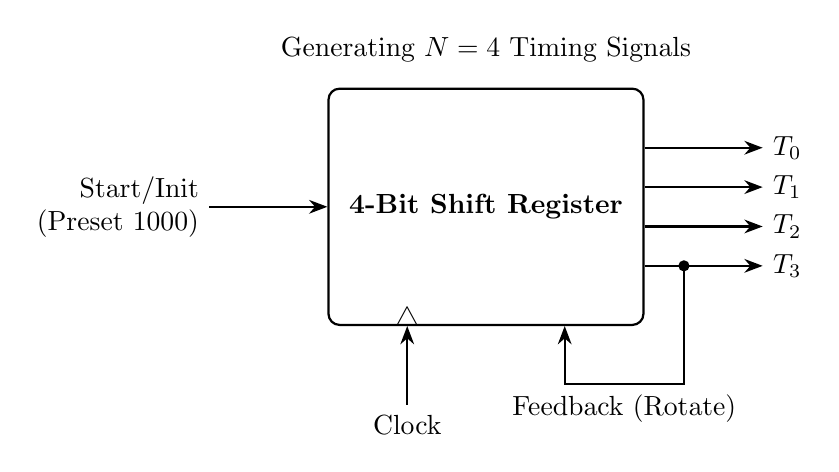
\begin{tikzpicture}[
    >=Stealth, 
    thick, 
    block/.style={draw, rectangle, minimum height=3cm, minimum width=4cm, fill=white, align=center, rounded corners},
]
    \node[block] (reg) {\textbf{4-Bit Shift Register}};
    
    % Inputs
    \draw[->] ($(reg.west) + (-1.5, 0)$) node[left, align=right] {Start/Init\\(Preset 1000)} -- (reg.west);
    
    \draw[->] ($(reg.south) + (-1, -1)$) node[below] {Clock} -- ($(reg.south) + (-1, 0)$);
    \node[above=-0.2cm of reg.south, xshift=-1cm] {$\triangle$};

    % Outputs
    \foreach \i in {0,1,2,3} {
        \coordinate (p\i) at ($(reg.east) + (0, {0.75 - \i*0.5})$);
        \draw[->] (p\i) -- ++(1.5, 0) node[right] {$T_\i$};
    }
    
    % Feedback
    \coordinate (last_out) at ($(reg.east) + (0.5, -0.75)$);
    \node[circ] at (last_out) {};
    
    \draw[->] (last_out) -- ++(0, -1.5) -| ($(reg.south) + (1, 0)$) node[pos=0.25, below] {Feedback (Rotate)};

    % Annotations
    \node[above=0.2cm of reg] {Generating $N=4$ Timing Signals};

\end{tikzpicture}
\end{document}
